\documentclass{report}
\usepackage{cmap}
\usepackage[T1]{fontenc}
\usepackage[utf8]{inputenc}
\usepackage[hungarian]{babel}
\usepackage[a4paper, left=20mm, top=20mm]{geometry}
\usepackage{listings}
\usepackage{graphicx}
\usepackage{float}
\usepackage{algorithmic}
\usepackage{amsmath}
\usepackage{textcomp}
\usepackage[hidelinks]{hyperref}
\setlength{\parindent}{0em}
\setlength{\parskip}{1em}

\hypersetup{
    colorlinks,
    citecolor=black,
    filecolor=black,
    linkcolor=black,
    urlcolor=black
}

\graphicspath{ {./chap1/media} {./chap2/media} {./chap3/media} {./chap4/media} {./chap5/media} {./chap6/media} {./chap7/media} {./chap8/media} {./chap10/media} }

\title{Számítógép architektúrák alapjai}
\author{Készítette: Simon Péter \thanks{Hallgatói jegyzet Durczy Levente előadásai alapján}}

\begin{document}

\maketitle
\tableofcontents

% Első előadás

\chapter{Alapfogalmak}

\section{Architektúra fogalma}
A számítógép architektúra fogalmat először Amdahl, az IBM mérnőke használta először a 360-as család bejelentésekor.
Definíciója szerint ez az a struktúra, amit a gépi kódú programozónak értenie kell, hogy helyes programot tudjon írni az adott gépre.
Tehát a regiszterek, memória, utasításkészlet, címzési módok és utasításkódok összessége, mind logikai, mind hardveres szinten.

\section{Számítási modellek}
A számítási modell a számításra vonatkozó alapelvek egy absztrakciója.
A számítási modelleket a következő absztrakciós jellemzőkkel írhatjuk le:
\begin{itemize}
    \item min hajtjuk végre a számítást (általában adatokon - adat alapú)
    \item hogyan képezzük le a számítási feladatot
    \item milyen módon vezéreljük a végrehajtási sorrendet
\end{itemize}

\subsection{A számítási modell, az architekrúra és a programnyelv kapcsolata}
Egy számítógép tervezését a számítási modellel kell kezdeni, ami meghatározza, hogy mit szeretnénk csinálni.
Ehhez szükség van egy specifikációs eszközre, amit a programnyelv képvisel (pl. Neumann modell megvalósítási eszköze a BASIC, Fortran).
Ezután jön az architektúra, ami a számítási modell implementációs eszköze, a "vas".
Ez hajtja végre az adott programnyelven definiált feladatokat.

\subsection{Számítási modellek csoportosítása}
\subsubsection{Számítási modelljük szerint}
\begin{itemize}
    \item szekvenciális
    \item párhuzamos
\end{itemize}

\subsubsection{Vezérlés meghajtása szerint}
\begin{itemize}
    \item vezérlés meghajtott
    \item adat meghajtott
    \item igény meghajtott
\end{itemize}

\subsubsection{Probléma leírása szerint}
\begin{itemize}
    \item procedurális
    \item deklaratív
\end{itemize}

Első sorban aszerint különböztetjük meg őket, hogy min hajtjuk végre a számítást.
Az adatalapú modellek:
\begin{itemize}
    \item Neumann modell
    \item adatfolyam modell
    \item applikatív modell (igénymeghajtott)
\end{itemize}
Az adatalapú modelleken kívül léteznek még objektum alapú, predikátum logika alapú, tudás alapú és hibrid modellek.
A mai processzorokban a Neumann és az adatfolyam modellek keverednek.

\subsection{Adatalapú modellek közös tulajdonságai}
\begin{itemize}
    \item az adatok általában típussal rendelkeznek (pl. 16 bit int) - vannak elemi és összetett adattípusok
    \item a típus meghatározza az adat értelmezési tartományát, értékkészletét és az elvégezhető műveleteket
\end{itemize}

\subsection{Neumann modell}
A Neumann-elvű számítógépek a számításokat adatokon hajtják végre, amiket egy változó értékű változókészlet képvisel.
A végrehajtási sorrend vezérlés meghajtott, tehát van egy statikus utasításszekvencia, amit egy speciális regiszter biztosít (program counter).
A program counter egy inkrementálódó változó, mindig a végrehajtandó utasításra mutat.
A végrehajtási sorrendtől vezérlési feladatokat ellátó utasításokkal lehet eltérni (pl. jump, if).

A Neumann elv követelményrendszere előírja változók létrehozását, adatmanipulációs és vezérlés átadási utasítások deklarálását.
Az ilyen nyelveket hívjuk imperatív (parancs) programnyelveknek (pl. C, Pascal, Assembly).

Ezeket a követelményeket az architektúra kielégíti, pl. lehetővé teszi, hogy a memóriában elhelyezkedő változók korlátlan számban módosíthatók legyenek a program futása során.
Ezen kívül biztosítja a megfelelő regisztereket az adatoknak és speciális regisztereket mint pl. program counter.

Az adatok és az utasítások a memóriában helyezkednek el.
A számítási feladat műveletek elemi műveletek sorozataként értelmezhető.
Egy számítási feladat leképezhető adat manipuláló utasítások sorozatával.
Az adat manipuláló utasítások az utasítások sorrendjében vannak végrehajtva, ezért ez egy vezérlés meghajtott modell.
A vezérlést a program counter biztosítja, a sorrendet a programozó határozza meg.
Az explicit vezérlés átadó utasításokkal lehet eltérni az implicit szekvenciától.

Következmények:
\begin{itemize}
    \item előzmény érzékenység: mivel az adatok változhatnak bármikor a végrehajtás során, a végrehajtás sorrendje nem mindegy
    \item alapvetően szekvenciális végrehajtást biztosít
    \item egyszerűen implementálható
    \item az adatmanipuláló utasítások nem szándékos állapotmódosulást okozhatnak (pl. overflow) - ezeket mellékhatásoknak hívjuk, kezelni kell őket
\end{itemize}

\subsection{Adatfolyam modell}
A számítást itt is adatokon hajtjuk végre, de:
\begin{itemize}
    \item az adatokat bemenő adathalmaz képviseli
    \item egyszeres értékadás lehetséges
    \item a megoldandó feladatot adatfolyam gráffal és input adatok halmazával képezzük le
    \item szakosodott végrehajtó egységeket használ
    \item a végrehajtást az adat vezérli - adatvezérelt, azaz az adat rendelkezésre állásakor azonnal működésbe lép a végrehajtó egység
\end{itemize}
% Második előadás
% FIXME: statikus vs dinamikus kezelés

\chapter{Függőségek}

\section{Bevezetés}
A függőségek gátolják a párhuzamos végrehajtást.

\section{Típusai}
\begin{itemize}
    \item adat
    \item vezérlés
    \item erősforrás
\end{itemize}

\section{Adat függőségek}
Probléma: az utasítás végrehajtáshoz egy előző utasítás eredményére van szükség.

\subsection{Csoportosítása}
\subsubsection{Jellege szerint}
\begin{itemize}
    \item utasítás szekvenciában (lineáris feldolgozás)
          \begin{itemize}
              \item valós függőség - nem teljesen megszüntethető (RAW - Read After Write)
                    \begin{itemize}
                        \item műveleti adatfüggőség
                        \item behívási adatfüggőség
                    \end{itemize}
              \item ál függőség - teljesen megszüntethető
                    \begin{itemize}
                        \item WAR - Write After Read
                        \item WAW - Write After Write
                    \end{itemize}
          \end{itemize}
    \item ciklusban
\end{itemize}
\subsubsection{Operandus típusa szerint}
\begin{itemize}
    \item regiszter
    \item memória
\end{itemize}

\subsection{Műveleti adatfüggőségek}
\paragraph{Probléma felvetés:} feltélezzük, hogy
\begin{itemize}
    \item a processzor 3 operandusos utasításokat használ
    \item 4 fokozatú futószalagos végrehajtás van (Fetch, Decode, Execute, WriteBack).
\end{itemize}
Ezekkel a feltételekkel két számot szeretnénk összeszorozni, az eredményt pedig megduplázni. Az utasításaink:
\begin{lstlisting}[language=Ant]
;I1
MUL r3,r2,1   ;r3 = r1 * r2
;I2
SHL r3        ;r3 * 2
\end{lstlisting}
Az utasítások végrehajtásának időbeli sorrendje:
\begin{center}
    \begin{tabular}{ c | c | c | c | c | c}
                           & t\textsubscript{1}   & t\textsubscript{2}      & t\textsubscript{3}   & t\textsubscript{4}    & t\textsubscript{5}    \\
        \hline
        I\textsubscript{1} & F\textsubscript{MUL} & D\textsubscript{r1, r2} & E\textsubscript{MUL} & W/B\textsubscript{r3} &                       \\
        \hline
        I\textsubscript{2} &                      & F\textsubscript{SHL}    & D\textsubscript{r3}  & E\textsubscript{SHL}  & W/B\textsubscript{r3}
    \end{tabular}
\end{center}
A probléma, hogy I\textsubscript{2} végrehajtása során, a dekódolási fázisban (t\textsubscript{3} időpillanat) szükség lenne az r3 regiszter értékére, viszont az csak t\textsubscript{4} időpillanatban áll elő (I\textsubscript{1} végrehajtásának writeback fázisában).
Tehát a futószalagos módszerrel párhuzamosított végrehajtás során műveleti adatfüggőség keletkezett, mivel az utasítások lehívása és végrehajtása között átfedés van.
Ilyenkor a műveletek elakadnak.
\paragraph{Megoldás:}egy speciális utasítás, a NOP (No Operand) használata az alábbi módon:
\begin{center}
    \begin{tabular}{ c | c | c | c | c | c | c | c}
                           & t\textsubscript{1}   & t\textsubscript{2}      & t\textsubscript{3}   & t\textsubscript{4}    & t\textsubscript{5}  & t\textsubscript{6}   & t\textsubscript{7}    \\
        \hline
        I\textsubscript{1} & F\textsubscript{MUL} & D\textsubscript{r1, r2} & E\textsubscript{MUL} & W/B\textsubscript{r3} &                     &                                              \\
        \hline
        I\textsubscript{2} &                      & F\textsubscript{SHL}    & NOP                  & NOP                   & D\textsubscript{r3} & E\textsubscript{SHL} & W/B\textsubscript{r3}
    \end{tabular}
\end{center}
\paragraph{Következmény:} a műveleteknek várakozniuk kell egymásra, két óraciklus késés keletkezik a futószalagon. Az ezeket követő utasításokhoz is be kell szúrni két NOP-ot, mivel a dekóder foglalt.
Ezt a jelenséget teljesen nem lehet megszüntetni, viszont a fékező hatást csökkenthetjük.
\paragraph{Kezelés:}operandus előrehozásával csökkenthető a fékező hatás, ez viszont extra hardvert igényel (hardveres, azaz dinamikus megoldás).
Extra hardver nélkül csak szoftveresen, azaz statikusan kezelhetjük a problémát.
Ilyenkor a compiler oldja meg a függőségek kezelését.
Általában előnyösebb a dinamikus megoldás.
\paragraph{Dinamikus megvalósítás:} az ALU-hoz tartozó rejtett regisztereket és az adatutakat a \ref{fig:operandus_elorehozas} ábra mutaja.
Alapesetben a MUL utasítás végrehajtása során az adat az r\textsubscript{1} és r\textsubscript{2} regiszterekből az src\textsubscript{1}, illetve src\textsubscript{2} regiszterekbe kerül, majd a művelet elvégzése után a rslt rejtett regiszteren keresztül visszaírásra kerül r\textsubscript{3}-ba.
Az adatút rövidítésének érdekében, extra hardver segítségével az rslt regiszter tartalmát közvetlenül visszavezethetjük az ALU egyik forrásregiszterébe. Ennek útja látható az ábrán pirossal.
Ekkor az utasítások végrehajtása az alábbi módon valósul meg:
\begin{center}
    \begin{tabular}{ c | c | c | c | c | c | c | c}
                           & t\textsubscript{1}   & t\textsubscript{2}      & t\textsubscript{3}   & t\textsubscript{4}    & t\textsubscript{5}    & t\textsubscript{6} & t\textsubscript{7} \\
        \hline
        I\textsubscript{1} & F\textsubscript{MUL} & D\textsubscript{r1, r2} & E\textsubscript{MUL} & W/B\textsubscript{r3} &                       &                                         \\
        \hline
        I\textsubscript{2} &                      & F\textsubscript{SHL}    & D                    & E\textsubscript{SHL}  & W/B\textsubscript{r3} &                    &
    \end{tabular}
\end{center}
Mivel már t\textsubscript{3} időpillanatban is rendelkezésre áll az SHL utasítás operandusa, két óraciklussal hamarabb kezdhető meg a művelet végrehajtása. Ezzel megszüntettük a késést.
Ezt a megoldást minden modern CPU használja.

\begin{figure}[H]
    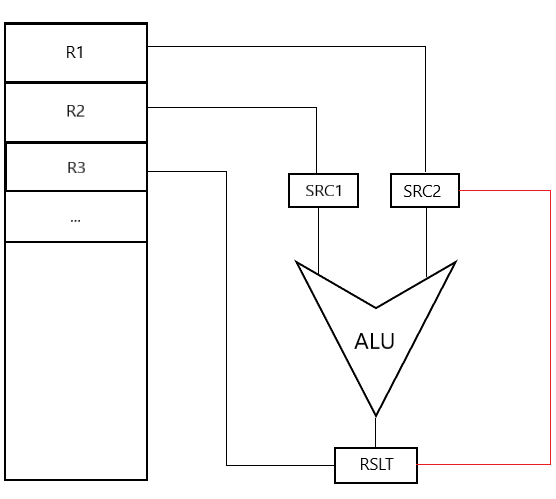
\includegraphics[width=0.6\textwidth]{operandus_elorehozas}
    \centering
    \caption{Az eredmény visszavezetése a forrás regiszterbe}
    \label{fig:operandus_elorehozas}
\end{figure}

\subsection{Lehívási adatfüggőség}
\paragraph{Probléma:} a regiszterekbe az operatív tárból (cache) töltjük be a szükséges adatokat, majd ezután a regiszterekből hívja le a végrehajtó egység (ALU).
A cache elérése viszont sok időt vesz igénybe.
Ennek látható az általános adatútja a \ref{fig:lehivas_elorehozas} ábrán, fekete vonallal jelölve.
\paragraph{Kezelés:} a folyamat gyorsítására extra hardvert alkalmazunk, amivel a cache-ből történő lehíváskor egyúttal a végrehajtó egységbe is betöltjük az adatot (piros vonal).
Így egy óraciklust megspórolhatunk.

\begin{figure}[H]
    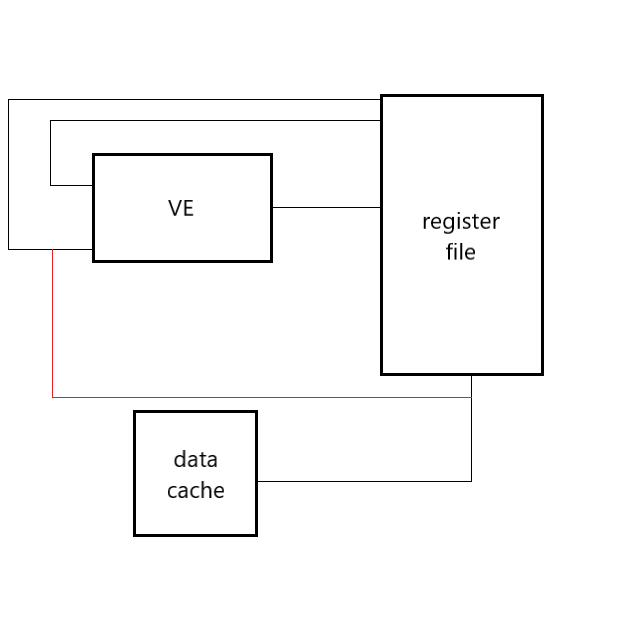
\includegraphics[width=0.6\textwidth]{lehivas_elorehozas}
    \centering
    \caption{A lehívott adat bevezetése a műveletvégző egységbe}
    \label{fig:lehivas_elorehozas}
\end{figure}

\subsection{WAR - Write After Read}

\paragraph{Probléma felvetés:} egy MUL utasítást egy ADD követ az alábbi módon:
\begin{lstlisting}[language=Ant]
    ;I1
    MUL r3,r2,1   ;r3 = r1 * r2
    ;I2
    ADD r2,r4,r5  ;r2 = r4 + r5
\end{lstlisting}
A szorzás (MUL) sokkal lassabb, mint az összeadás (ADD), ezért előfodulhat, hogy a párhuzamos
végrehajtás során I\textsubscript{2} hamarabb lefut, mint hogy I\textsubscript{1} betöltse a forrás operandust.
Mivel I\textsubscript{2} módosította I\textsubscript{1} bemeneti operandusát, a MUL utasítás hibás eredményt fog adni.
Következménye, hogy sérül a szekvenciális konzisztencia.
\paragraph{Megoldás:} r\textsubscript{2} tartalmát egy ideiglenes regiszterbe irányítjuk (pl. r\textsubscript{23}).
Ekkor az assmebly utasítások így néznek ki:
\begin{lstlisting}[language=Ant]
    ;I1
    MUL r3,r2,1   ;r3 = r1 * r2
    ;I2
    ADD r23,r4,r5 ;r23 = r4 + r5
\end{lstlisting}
Az r\textsubscript{23}$\,\to\,$r\textsubscript{2} hozzárendelést nyilvántartjuk, majd amikor a MUL utasítás végzett, visszaírjuk r\textsubscript{23} tartalmát r\textsubscript{2}-be.
Az átmeneti (átnevezési) regiszterek tulajdonságai:
\begin{itemize}
    \item új, önálló, de rejtett,
    \item saját címtartománnyal rendelkezik,
    \item a programozó számára traszparens,
    \item extra hardvernek számít.
\end{itemize}

\paragraph{Megjegyzés:} a regiszterkészletek csoportosítása:
\begin{itemize}
    \item architekturális: programozó használja,
    \item átnevezési: a vezérlés használja az álfüggőségek feloldására.
\end{itemize}

\subsection{WAW - Write After Write}
\paragraph{Probléma felvetés:} egy MUL utasítást egy ADD követ az alábbi módon:
\begin{lstlisting}[language=Ant]
    ;I1
    MUL r3,r2,1   ;r3 = r1 * r2
    ;I2
    ADD r3,r4,r5  ;r3 = r4 + r5
\end{lstlisting}
A szorzás (MUL) sokkal lassabb, mint az összeadás (ADD), ezért előfodulhat, hogy a párhuzamos
végrehajtás során I\textsubscript{1} később fut le, mint I\textsubscript{1}.
Mivel az eredményt ugyanabba a regiszterbe írják, ebben az esetben I\textsubscript{1} felülírja I\textsubscript{2} eredményét az r\textsubscript{3}-ban.
Ezzel sérül a szekvenciális konzisztencia.
\paragraph{Megoldás:} r\textsubscript{3} átirányítása egy átnevezési regiszterbe, az előbb leírt módon.

\subsection{Ciklusbeli függőség}

\paragraph{Probléma felvetés:}
egy ciklusban az előző iterációban kiszámolt adatot használunk fel, például:
\begin{algorithmic}
    \FOR{$i=2$ to $n$}
    \STATE X\textsubscript{i}$\leftarrow$A\textsubscript{i} * X\textsubscript{i-1} + B\textsubscript{i}
    \ENDFOR
\end{algorithmic}
\paragraph{Kezelés:} ez egy erős függőség, hardveresen nehezen feloldható. Megoldás az algoritmus áttervezése.

\section{Vezérlés függőségek}
Elágazások esetén léphetnek fel. Itt a statikus és dinamikus kezelésnek eltérő jelentése van, mint az adatfüggőségeknél. A statikus kezelés itt egy állandó, mindig alkalmazható eljárást jelent, míg a dinamikus kezelés az adott programtól függ.
\paragraph{Probléma felvetés:} az alábbi utasítássorozatban a feltétlen ugrás (JMP) egy SHL utasításra mutat:
\begin{lstlisting}[language=Ant]
    DIV
    MUL
    JMP ; SHL-re mutat
    ADD
    ...
    SHL
\end{lstlisting}
Ekkor a kritikus utasítások így követik egymást időben:
\begin{center}
    \begin{tabular}{ c | c | c | c | c | c | c }
            & t\textsubscript{1}   & t\textsubscript{2}   & t\textsubscript{3}   & t\textsubscript{4} & t\textsubscript{5} & t\textsubscript{6} \\
        \hline
        MUL & F\textsubscript{MUL} & D                    & E                    & W/B                &                    &                    \\
        \hline
        JMP &                      & F\textsubscript{JMP} & D                    & E                  & W/B                                     \\
        \hline
        ADD &                      &                      & F\textsubscript{ADD} & D                  & E                  & W/B
    \end{tabular}
\end{center}
A JMP utasítás az Execute fázisban állítja át a Program Countert, ezzel végzi el az ugrást.
A futószalag végrehajtás miatt azonban ekkorra már a következő utasítás, az ADD is lehívásra került, sőt, előfordulhat, hogy az azt követő utasítás is.
Ezek viszont fölösleges lépések. Ritkább esetekben a JMP-t követő utasítás be is fejeződhet, mire az ugrás végrehajtásra kerül, ami veszélyezteti az architekturális regisztertartalmakat.
\paragraph{Megoldás:} a probléma kezelése statikus, dinamikus, vagy spekulatív (branch prediction) módon történhet.
\paragraph{Kezelés utasítások átrendezésével (dinamikus):} compiler segítségével történő optimalizálás. A compiler megpróbálja átrendezni az utasítások sorrendjét.
Az előző kódrészlet optimalizált változata:
\begin{lstlisting}[language=Ant]
    JMP ; SHL-re mutat
    MUL
    DIV
    ADD
    ...
    SHL
\end{lstlisting}
Az optimalizálás utáni végrehajtási sorrend:
\begin{center}
    \begin{tabular}{ c | c | c | c | c | c | c | c }
            & t\textsubscript{1}   & t\textsubscript{2}   & t\textsubscript{3}   & t\textsubscript{4}   & t\textsubscript{5} & t\textsubscript{6} & t\textsubscript{7} \\
        \hline
        JMP & F\textsubscript{JMP} & D                    & E                    & W/B                  &                    &                                         \\
        \hline
        MUL &                      & F\textsubscript{MUL} & D                    & E                    & W/B                                                          \\
        \hline
        DIV &                      &                      & F\textsubscript{DIV} & D                    & E                  & W/B                                     \\
        \hline
        SHL &                      &                      &                      & F\textsubscript{SHL} & D                  & E                  & W/B
    \end{tabular}
\end{center}
A sorrend megváltoztatásával elértük, hogy amíg az ugrás végre nem hajtódik (t\textsubscript{3}), csak olyan utasításokat hívunk le, amiknek még az ugrás előtt kell lefutniuk.
Mire az ADD utasításhoz elérnénk, felülíródik a PC és a megfelelő utasítás hívódik le (SHL).
A módszer hátránya, hogy hatékonysága a futószalag fokozatok számának növelésével rohamosan csökken.
\paragraph{Kezelés NOP utasításokkal (statikus):} a JMP utasítás mögé egy vagy több NOP utasítás kerül be.
Ez a futószalag várakoztatását jelenti, amíg elő nem áll az ugráshoz szükséges PC. Ez az ún. ugrási buborék, nagysága $n-1$, ahol $n$ a futószalag fokozatok száma.

% Harmadik előadás

\chapter{Időbeli párhuzamosság: futószalag CPU-k}

\section{Bevezetés}
A futószalagos (pipeline) végrehajtás lényege, hogy egy utasítást több részre osztunk (általában fetch, decode, execute, writeback), majd ezeket a részeket külön, egymással párhuzamosan hajtjuk végre (\ref{fig:pipeline} ábra).
Az utasítások $n$ részre osztásával elméletileg a sebesség $n$-szeresére növekszik.
\begin{figure}[h]
    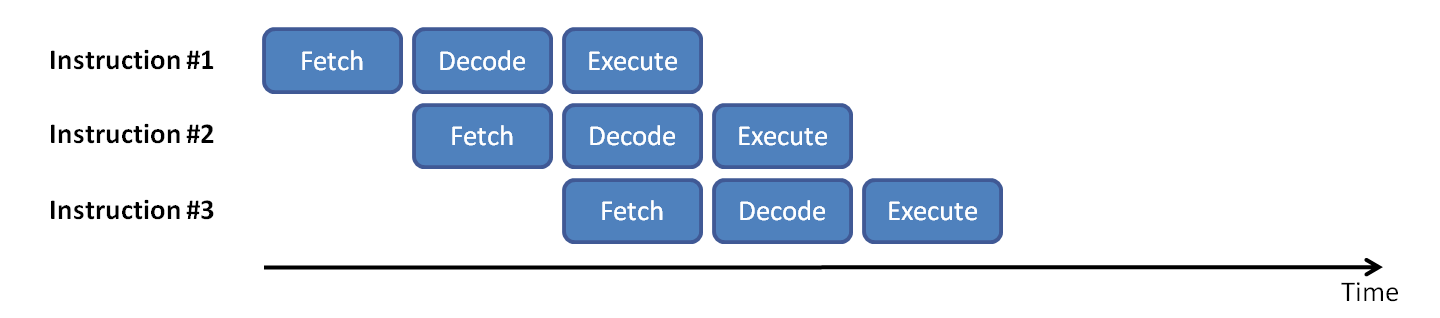
\includegraphics[width=0.6\textwidth]{pipeline}
    \centering
    \caption{Futószalagos végrehajtás}
    \label{fig:pipeline}
\end{figure}
\paragraph{A teljesítmény gátjai:} a gyakorlatban nem mindig valósul meg a fokozatok számának növekedésével arányos gyorsulás.
A végrehajtást a függőségek (adat, vezérlés, erőforrás) lassítják. A függőségek oka a sok párhuzamosan futó utasítás ($n+1$, ahol $n$ a fokozatszám).
\paragraph{A hatékonyság maximalizálása:}a tapasztalat szerint a hatékonyság kb. 15-30 fokozatú futószalag esetén maximalizálható, efölött a függőségek miatt már csökken a teljesítmény.
Ez az általános célú alkalmazásokra igaz, a mai általános processzorokban kb. 20 fokozat van. Speciális feladatokra (ahol kevés a függőség) használható superpipeline CPU, ami akár 200 fokozatú is lehet.

\section{Történeti áttekintés}
\begin{itemize}
    \item Intel 80486: 3 fokozat, de már külön lebegőpontos futószalag
    \item Intel Pentium (P5): 5 fokozat
    \item Intel Pentium III (P6): 11-17 fokozat
    \item Intel Pentium IV (Netburst): 20-31 fokozat
    \item Intel Core 2 (újratervezett P6, több mag): általában 14 fokozat
    \item Intel Core i: 16-20 fokozat
\end{itemize}

\section{Gyakorlati példa - az Intel Atom CPU}
Az Intel Atom processzor a 2000-es években jelent meg, 16 fokozatú futószalagot használ.
A processzor CISC (Complex Instruction Set Computing) architektúrájú, azaz egy utasításon belül nem csak a regiszterekből, hanem a memóriából, vagy a gyorsítótárból is képes adatot lehívni.
\paragraph{Az Intel Atom fokozatai:}
\begin{itemize}
    \item 1-3. fokozat: instruction fetch (IF)
    \item 4-6. fokozat: instruction decode (ID)
    \item 7-8. fokozat: instruction dispatch (SC - Switch Context, IS - Instruction Schedule)
    \item 9. fokozat: source operand read (IRF - Instruction Register File)
    \item 10-12. fokozat: data cache access, CISC architektúrához szükséges (AG - Address Generation, DC\textsubscript{1} - Data Cache 1, DC\textsubscript{2} - Data Cache 2)
    \item 13. fokozat: execute
    \item 14-15. fokozat: exception + multitask handling (FT\textsubscript{1} - Fault Tolerant 1, FT\textsubscript{2} - Fault Tolerant 2)
    \item 16. fokozat: commit, ez a visszaírás (W/B vagy DC\textsubscript{1})
\end{itemize}
\paragraph{Következmény:} ez egy tisztán futószalag elvű processzor, ami teljesítményben visszalépést jelentett a korábbi architektúrákhoz képest.
Előnye az alacsony fogyasztás, ezért főleg mobil eszközökbe használták az Atom CPU-kat.

\section{Futószalagos feldolgozás előfeltételei (2 fokozat esetén)}
Az ideális futószalag megvalósítható, ha
\begin{itemize}
    \item a számítógép 2 db egymástól független végrehajtó egységgel rendelkezik,
    \item az egyik fokozat kimenete a másik fokozat bemenete,
    \item mindkét fokozat végrehajtási ideje azonos,
    \item a fokozatok szinkronizáltak, órajelre kapják az inputot, és egyetlen óraciklus alatt elvégzik a feladatukat.
\end{itemize}
Ekkor $t=\frac{T}{2}$, ahol $T$ a szekvenciális végrehajtási idő és $t$ a futószalagos végrehajtási idő.

\section{Függőségek kezelése}
\begin{itemize}
    \item Operandus előrehozással:
    \begin{itemize}
        \item Minden architektúránál használják.
        \item Részletesen: \ref{fuggosegek}. fejezet.
    \end{itemize}
    \item Újrafeldolgozással:
    \begin{itemize}
        \item Leggyakrabban az execute fokozat egymás után többszöri végrehajtását jelenti.
        \item Pl. szorzásnál az ismétlődő összeadásokhoz használható.
        \item A futószalag feldolgozást lassítja, de összességében jobb teljesítményt biztosít.
    \end{itemize}
\end{itemize}

\section{Típusai}
\begin{enumerate}
    \item Előlehívás (overlapping)
    \item Vektor CPU-k (60-as évek)
    \item Teljes pipeline
\end{enumerate}

\subsection{Előlehívás}
A visszaírás során történik meg a következő utasítás lehívása:
\begin{center}
    \begin{tabular}{ c | c | c | c | c | c | c | c }
        & t\textsubscript{1} & t\textsubscript{2} & t\textsubscript{3} &t\textsubscript{4} & t\textsubscript{5} & t\textsubscript{6} & t\textsubscript{7} \\
        \hline
        I\textsubscript{1} & F & D & E & W/B \\
        \hline
        I\textsubscript{2} &   &   &   & F & D & E & W/B
    \end{tabular}
\end{center}
\paragraph{Előnyök:}
\begin{itemize}
    \item 4 óraciklus helyett csak 3 kell egy utasításhoz, így a teljesítmény 25\%-al nő, valamint
    \item nincsenek függőségek, mivel a forrás operandus beolvasásakor (t\textsubscript{5}) már megvan az előző utasítás eredménye (t\textsubscript{4}).
\end{itemize}
\paragraph{Hátrány:} nem túl nagy mértékű gyorsulás.

\subsection{Vektor CPU}
Csak az execute fokozat működött futószalagszerűen.

\subsection{Teljes pipeline}
A futószalagos feldolgozás kiterjesztése a teljes folyamatra:
\begin{center}
    \begin{tabular}{ c | c | c | c | c | c  }
        & t\textsubscript{1} & t\textsubscript{2} & t\textsubscript{3} &t\textsubscript{4} & t\textsubscript{5} \\
        \hline
        I\textsubscript{1} & F & D & E & W/B \\
        \hline
        I\textsubscript{2} &   &  F & D & E & W/B
    \end{tabular}
\end{center}

\section{Logikai futószalagok} \label{logikai_futoszalag}
Az eltérő utasítások eltérő felépítésű futószalagokat igényelnek, ezért egy processzor több futószalagot is tartalmaz.
A cél a funkcionális kialakítás. Példák különböző funkciókat ellátó futószalagokra:
\begin{itemize}
    \item aritmetikai: F, D, E, W/B
    \begin{itemize}
        \item fixpontos
        \begin{itemize}
            \item egyszerű: +, -, léptetés, ...
            \item összetett: *, /, ...
        \end{itemize}
        \item lebegőpontos
    \end{itemize}
    \item ugró (branch): F, E
    \item LOAD / STORE
\end{itemize}
\paragraph{Az utasítások értelmezése:} az utasításokat két szinten értelmezhetjük, pl. a fetch utasítás két szintje a következő:
\begin{enumerate}
    \item Fetch
    \item MAR $\leftarrow$ PC\\
    MDR $\leftarrow$ [MAR] \\
    IR $\leftarrow$ MDR \\
    PC $\leftarrow$ PC+1
\end{enumerate}

\section{Fizikai megvalósítás}
Alkalmazásuk alapján megkülönböztetünk univerzális és dedikált futószalagokat.
Az univerzális minden művelet elvégzésére alkalmas, míg a dedikált speciális műveletekre képes.
Hardveres szempontból az univerzális futószalag előnytelen, mivel sok tranzisztorra van szükség, a kialakítása bonyolult és drága, ráadásul a végrehajtás lassú.
Ezért általában a \ref{logikai_futoszalag}. részben leírt dedikált (egy adott funciót ellátó) futószalagokat építenek a processzorokba.
Az eredmény kevesebb logikai kapu, így gyorsul a végrehajtás (a bemenettől a kimenetig gyorsabban átérnek az elektronok).
\paragraph{Megjegyzés:} a futószalag sebességét általában a leglassabb fokozat sebessége határozza meg, tehát a tervezési cél a megközelítőleg azonos sebességű fokozatok létrehozása.
\paragraph{Fokozatok kialakítása:} a fokozatok előtt előválasztó (puffer) regiszterek vannak. Ezek a felhasználó számára láthatatlanok, az adat először ezekbe töltődik be.
Ezekből a regiszterekből kerül aztán a végrehajtó egységbe az adat, majd az utasítás elvégzése után szintén puffer regiszterekbe kerül a kimenet.
A puffer regiszterek szükségesek, mivel a gyakorlatban egy fokozat nem mindig végez egy óraciklus alatt.
Az ebből adódó várakozás során ezekben a regiszterekben tárolódik az adat.
Ennek a kialakítása látható a \ref{fig:fokozat}. ábrán. A későbbiekben a végrehajtó egységekből egymás mellé többet is helyeztek, így megvalósítva a térbeli párhuzamosságot (\ref{fig:fokozat_parhuzamos}. ábra).
\begin{figure}[h]
    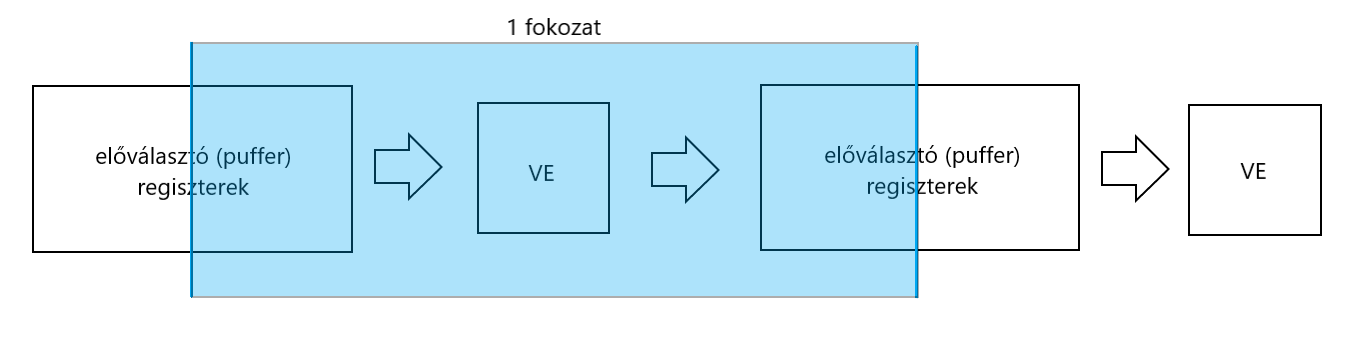
\includegraphics[width=0.6\textwidth]{fokozat}
    \centering
    \caption{A fokozatok felépítése}
    \label{fig:fokozat}
\end{figure}
\begin{figure}[h]
    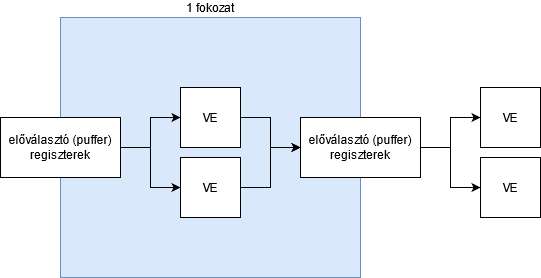
\includegraphics[width=0.6\textwidth]{fokozat_parhuzamos}
    \centering
    \caption{A végrehajtó egységek párhuzamosítása}
    \label{fig:fokozat_parhuzamos}
\end{figure}

\subsection{Példa: a PowerPC 604}
A PowerPC 604-es processzorban egymással párhuzamosan több dedikált futószalag is működött (\ref{fig:powerpc604} ábra).
A fetch és decode fokozatok minden óraciklusra lehívtak egy utasítást, és a megfelelő futószalagba töltötték.
Így a CPU képes volt egymással párhuzamosan több utasítást is végrehajtani (akár 4-et is).
Mivel előfordulhatott, hogy a később lehívott és betöltött utasítás végzett hamarabb (pl. elsőként egy FP, másodikként egy FX utasítás $\rightarrow$ FX hamarabb végez), szükséges volt egy konzisztencia fokozat (CO) bevezetése.
Az utasítások címkézésre kerültek, a sorrendet a CO biztosította.
A párhuzamosság miatt szükség volt a fokozatok közötti várakoztatásra, ez az interlock funkció.
\paragraph{Megjegyzés:} az Intel 80486 és az első Pentium csak 2 utasítás futószalaggal rendelkezett. A mai Core i architectúrák magonkánt általában 6-8 futószalagot alkalmaznak.
\label{powerpc604}
\begin{figure}[H]
    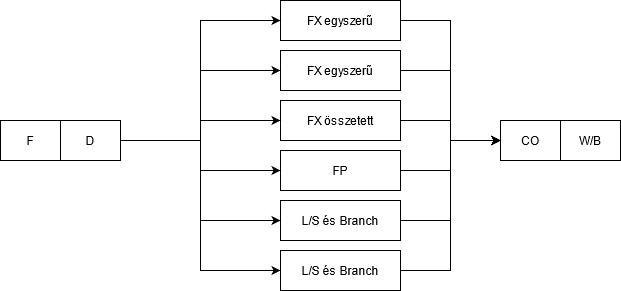
\includegraphics[width=0.6\textwidth]{powerpc604}
    \centering
    \caption{A PowerPC 604 futószalagja}
    \label{fig:powerpc604}
\end{figure}

\section{RISC és CISC architektúrák}
Az utasításkészlet (tervezési stratégia) alapján kétféle architektúrát különböztetünk meg:
\begin{itemize}
    \item RISC: Reduced Instruction Set Computing - csökkentett utasításkészletű architektúra és
    \item CISC: Complex Instruction Set Computing - bővített utasításkészletű architektúra.
\end{itemize}
Mindkettő használatban van napjainkban.
\subsection{Történeti áttekintés}
Az első CPU-k kevés utasítással rendelkeztek (RISC), majd a 70-es években az egyre több funkció és bonyolultabb utasítások miatt ez a szám növekedett (CISC).
A 80-as években rájöttek, hogy a sok utasítás ugyan megkönnyíti a programozást, de a címzés bonyolultsága miatt káros hatással van a teljesítményre.
Ez vezetett a RISC architektúrák újbóli megjelenéséhez.

\subsection{RISC}
\paragraph{Példa:} a mobil eszközök ARM (Advanced RISC Machine) processzorai RISC architektúrájúak.
\paragraph{Tulajdonságai:}
\begin{itemize}
    \item Kis számú (50-150) utasítással rendelkezik $\rightarrow$ címzési módok egyszerűsödése.
    \item Nincs olyan utasítás, ami a LOAD/STORE-t aritmetikával kombinálja (nem lehet egyszerre betölteni az adatot és végrehajtani a műveletet).
    \item Minden műveletvégző utasítás regisztereket használ $\rightarrow$ memóriából vagy gyorsítótárból nem lehet dolgozni.
    \item Memória vagy cache elérés csak LOAD/STORE utasításokkal történhet.
    \item Nagy számú regiszterkészlet (mivel minden művelethez regiszterekre van szükség).
    \item Általában 3 operandusos utasítások $\rightarrow$ az eredmény nem írja felül a bemeneti regisztert, hanem külön regiszterbe kerül.
    \item Minden utasítás hossza egyforma (pl. 128 bit) $\rightarrow$ könnyebb a futószalagos feldolgozás.
    \item A fordítóprogramok bonyolultabbak a kevés utasítás miatt.
    \item Általában huzalozott (hardveres) az utasítás feldolgozás (decode).
    \item Utasítás végrehajtás általában egy óraciklust vesz igénybe (cél az egyforma ciklusidő).
\end{itemize}
\paragraph{Előnye:} általában gyorsabb végrehajtás a CISC architektúrákhoz képest.
\paragraph{Hátránya:} a bonyolultabb feladatokat instrukció szekvenciákkal kell megoldani.
Ez a fordításnál okoz problémát, növelheti a program méretét.

\subsection{CISC}
\paragraph{Példa:} a 80-as években elterjedt Intel 80386-os egy tisztán CISC architektúra.
\paragraph{Tulajdonságai:}
\begin{itemize}
    \item Nagy számú utasításkészlet (több száz).
    \item A sok utasítás nagy belső mikroprogramtárat igényel.
    \item Sokféle címzési mód (tartalmaz típus címzési módot is) és sokféle utasítás.
    \item Változó méretű (akár összetett) utasítások $\rightarrow$ a dekódolónak nem csak dekódolni kell az utasítást, hanem azonosítani is az utasítás végét (tudnia kell, hogy hol fejeződik be). Ezt hívják utasítás határra illesztésnek, plusz hardvert és időt igényel.
    \item Közvetlen memória elérés lehetsége $\rightarrow$ a második operandus lehet memória vagy cache cím is.
    \item Két operandusos utasítások $\rightarrow$ az első operandus felülíródik az eredménnyel.
    \item Az előző kettőből következik, hogy az első operandus nem lehet memória/cache cím, mivel az eredmény memóriába írása nagyon lelassítaná a működést.
    \item Az utasítások feldolgozása több ciklusidő lehet $\rightarrow$ bonyolultabb feldolgozás.
    \item Egyszerűbb a gépi kódú programozás a sokféle utasítás miatt (egyszerűbb fordítóprogramok).
    \item Egy utasításban több elemi műveletet is végre tud hajtani.
    \item Az utasítások folyamatosan bővültek, így a régi programokkal visszafelé kompatibilis maradt.
    \item A futószalag fokozatok között sebesség különbség lehet $\rightarrow$ feloldására interlock funkciót használnak (részletesen: \ref{powerpc604}).
    \item Általában a memória elérés miatt +2 fokozat szükséges a RISC-hez képest (AG - címszámítás és cache elérés).
\end{itemize}
\paragraph{Előnyei:} kompatibilitás a régi programokkal, egyszerűbb compilerek.
\paragraph{Hátránya:} bonyolultabb, lassabb végrehajtás.

\subsection{Hibrid CISC}
\paragraph{Példa:} az x86-os architektúra ISA-t (Instruction Set Architecture) használ, ami egy hibrid CISC architektúra.
\paragraph{Tapasztalat:} megfigyelték, hogy a CISC processzorok az idő 80\%-ában az utasítások mindössze kb. 20\%-át használják.
\paragraph{Optimalizálás:} a feldolgozás gyorsítása érdekében kialakítottak a CISC architektúrán belül egy RISC magot.
Ez a megoldás minden mai (Core i) architektúrában megjelenik.

\subsection{Hibrid RISC}
A mai ARM processzorok sem tisztán RISC architektúrák, hanem CISC jellegű utasításokkal vannak kibővítve (pl. az ARM Thumb, ami egy tömörített utasításkészlet).

\section{Következmények}
A futószalagos feldolgozás következményei:
\begin{itemize}
    \item Jelentősen felgyorsult az utasítások lehívása és az operandusok betöltése.
    \item Amíg a processzorok feldolgozási sebessége jelentősen nőtt, a memória sebessége kevésbé (ez a jelenség a sebességolló) $\rightarrow$ cache bevezetése (IBM - 1968, Intel - 80-as évek). A cache előnye, hogy a gyakran használt operandusok gyorsan elérhetők.
    \item Maximális végrehajtási sebesség: 1 utasítás / ciklus (további növekedés kibocsájtási párhuzamossággal vagy utasításon belüli párhuzamossággal lehetséges).
    \item A vezérlés átadási utasítások kifinomult technikája szükséges (függőségek miatt).
    \item Az elágazás kezelés bonyolódik.
\end{itemize}

\subsection{Elágazások kezelése}
\subsubsection{Korai RISC gépek}
Kezelés ugrási buborékkal.
\subsubsection{Korai CISC gépek}
A dekódoló fokozatba építették a címszámító és a logikai komparáló egységet, így a dekódolási ciklus végére előáll az ugrási cím.
\subsubsection{Későbbi CISC gépek (futószalag CPU-k és első generációs szuperskalár architektúrák)}
Kezelés fix előrejelzéssel, pl. mindig ugrik.
Ezzel a megoldással az ugrási cím előre kiszámításra kerül és megkezdődik az ugrási címen lévő utasítások lehívása.
Ha mégse kell ugrani, az utasításokat visszatörli és az eredeti helyen folytatódik a végrehajtás.
Előnye, hogy kiküszübölte az ugrási buborékot, növekszik a teljesítmény.
Korlátja, hogy ha nagy látenciával rendelkező műveletet kellett végrehajtani az ugrási feltételben, az blokkolta a kibocsájtást.
Ilyen megoldást használ például az Intel 80486-os CPU.
\subsubsection{Második generációs szuperskalár architektúrák}
A CPU a dekódolási folyamatok egy részét már akkor elvégzi, amikor az utasításokat az L1 cache-be írja.
Az előre elvégzett feladatok:
\begin{itemize}
    \item utasítás típusazonosítás
    \item ugrások felismerése
    \item utasításhossz meghatározása (szükséges, mivel CISC-nél változó az utasításhossz)
    \item spekulatív elágazásbecslés
    \begin{itemize}
        \item regiszterátnevezéssel
        \item átrendező puffer (Intel: ROB - ReOrder Buffer)
    \end{itemize}
\end{itemize}

\section{Összegzés}
A fejezetben felsorolt módszerekkel elérték a futószalag elvű processzorok teljesítményének korlátait.
A további gyorsítás érdekében párhuzamos kibocsájtást kellett alkalmazni, így jöttek létre a szuperskalár processzorok.
% Második előadás

\chapter{Nagy teljesítményű, két foglalatos szerver processzorok fejlődése}

\section{Szerver platformok osztályozása}
A szerver rendszerek feloszthatók egy processzoros (UP) és több processzoros platformokra.
A több processzoros platformok feloszthatók két foglalatos (2S/DP), négy vagy nyolc foglalatos (4S, 8S) és nyolcnál több foglalatos rendszerekre.
A piac nagy részét a két processzoros szerverek teszik ki (kb. 80\%), ezért részletesebben ezekkel foglalkozunk.

\section{Méret, tranzisztorok}
A 2S szerver processzorok nagy méretűek, sok tranzisztort tartalmaznak.
A 2000-es évek közepén a Pentium 4 szerver processzorok még viszonylag kevés tranzisztorból álltak (125 millió), ezért elég volt kb 1 cm\textsuperscript{2}-es lapka.
A magok számának növekedésével egyre több tranzisztor kellett, a Skylake (2017) processzoroknál már 8 milliárd.
Még újabb CPU-knál nincs információ.
Ezzel együtt a lapkaméret is tovább nőtt, a mai lapkáknál 8 cm\textsuperscript{2} körüli.

Mivel a lapkák gyártása nagyon komplex, nagyobb méretű lapkáknál több hiba előfordulhat, ezért alacsonyabb lesz a kihozatali arány.
A lapkák méretét így a gazdasági hatékonyság is meghatározza.

\section{Fogyasztás}
A HEDT processzoroknál is nagyobb fogyasztással kell számolni a szerver processzoroknál, 130-tól 200 W felettig mennek.

\section{Lábak száma}
A szerver processzorok sok lábbal kapcsolódnak a foglalatokhoz, amik precíz gyártást igényelnek.

\section{Magok száma}
A szerver alkalmazások általában jól párhuzamosíthatók, így a processzorok a lehető legtöbb magot implementálják.
A Pentium 4 szerver processzoránál még csak 1 mag volt, de később 28-ig növekedett a magok száma.

\section{Intel Cascade Lake 9200-AP}
Ez a 2x28, azaz 56 magos processzor az Intel válasza volt az AMD 64 magos EPYC Rome processzoraira.
Az AMD 2017-ben adta ki ezt a processzort, ami valós konkurenciát állított az Intelnek, ami 2015 környékén még nagyrészt egyeduralkodó volt a szervereknél.
Ezért az Intel két 28 magos lapkát tett egy foglalatba, és BGA (Ball Grid Array) tokozással látta el, ami forrasztásra készült.
A forrasztás miatt nem voltak külön megvásárolhatók, csak OEM-ek kapták meg.

A két lapka egybecsomagolása miatt egy két foglalatos rendszer gyakorlatilag 4 processzort jelent.

\section{Magszámok és tranzisztorok növekedése}
A kétfoglalatos szerver CPU-k esetében kb 2 évente duplázódott a magok száma (\ref{fig:core}. ábra).

\begin{figure}[H]
    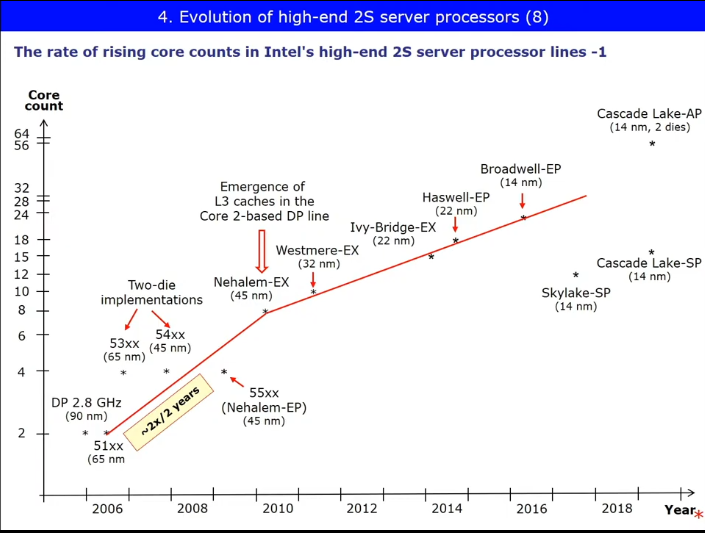
\includegraphics[width=0.8\textwidth]{core}
    \centering
    \caption{Intel 2S szerver processzorok magszámának fejlődése}
    \label{fig:core}
\end{figure}

Ez összhangban van a Moore-szabállyal, ami szerint a tranzisztorok száma két évente duplázódik.
Az utóbbi években viszont lelassult a fejlődés, már csak négy évente duplázódott a magok száma.
Ennek egyik oka az L3 cache megjelenése, ami elfoglalja a lapka jelentős részét, mivel nagyon sok tranzisztor kell a működéséhez.
A technológi változása miatt a Moore törvénnyel ellentétben az Intel már csak 4 évente tudta duplázni a tranzisztorok számát (\ref{fig:transistor}. ábra).
Ennek az oka, hogy a sok tranzisztor disszipációját kezelni kell, ami korlátozza a fejlődést.

\begin{figure}[H]
    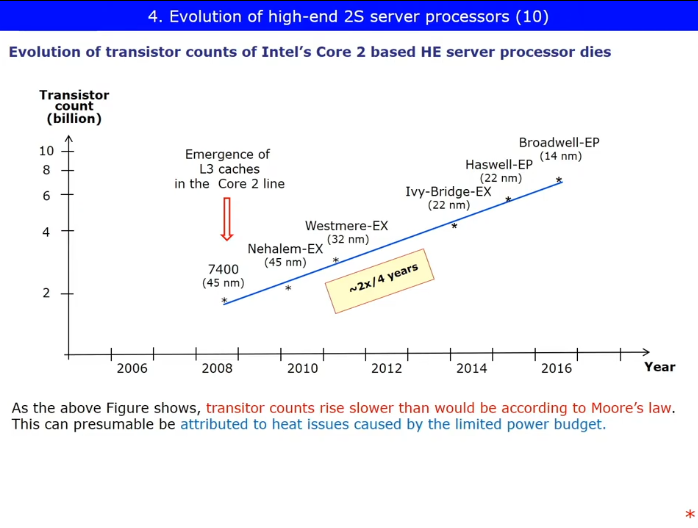
\includegraphics[width=0.8\textwidth]{transistor}
    \centering
    \caption{Intel 2S szerver processzorok tranzisztorszámának fejlődése}
    \label{fig:transistor}
\end{figure}

\subsection{Kivételek}
Néhány processzor az ábrán nem illik a fejlődési görbére, ezek az AMD konkurenciára adott válaszoknak köszönhetők.

\section{Memória sebességek fejlődése}
A memória sebességeknél adatátviteli rátával jellemezzük őket, mivel a frekvencia nem azonos az átviteli sebességgel a DDR (Double Data Rate) memóriák esetében.

\begin{figure}[H]
    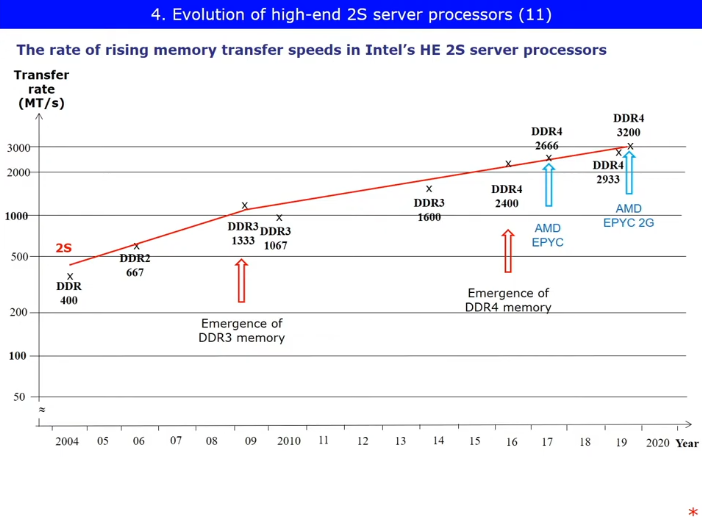
\includegraphics[width=0.8\textwidth]{mem}
    \centering
    \caption{Memória sebességek fejlődése}
    \label{fig:mem}
\end{figure}

A \ref{mem}. ábrán látható, hogy a DDR és DDR2-es memóriák gyorsabban fejlődtek, mint a DDR3 és DDR4 memóriák.
Az első szakaszban egy duplázódáshoz 4 év kellett, DDR3 óta pedig már 8.
Ennek oka a DDR3-as memóriák jóval komplexebb felépítése, ami lassította a fejlődést.
A magok száma tehát gyorsabban növekedett, mint a memóriák sebessége, ami konfliktusforrás.

Szerverek esetében elvárás, hogy az egymástól függetlenül működő magokat azonos memória sávszélességgel kell ellátni.
Tehát a sávszélességet lineárisan skálázni kell a magszámmal együtt.
A foglalatonkénti sávszélesség kiszámítása:
\begin{equation}
    BW/core = n_M*w*T_M/n_C
\end{equation}
ahol:
\begin{itemize}
    \item n\textsubscript{M}: memória csatornák száma
    \item w: memória csatorna szélessége (pl. 8 byte)
    \item T\textsubscript{M}: memória átviteli rátája (pl. 2.4 GT/s)
    \item n\textsubscript{C}: magok száma
\end{itemize}

Probléma, hogy a transzfer ráta lassabban nő, mint a magok száma, tehát $T_m/n_C$ folyamatosan csökken.
Megoldás a memória csatornák számának növelése.
Ez azonban elég komplex feladat.

A magonkénti memória sávszélességnél referenciának tekinthető a Pentium 4 DP rendszer, a fejlesztési cél ehhez az értékhez tartani.

% Hetedik előadás

\chapter{Lebegőpontos és BCD számok}

\section{Bevezetés}
A lebegőpontos számok szükségesek, mivel:
\begin{itemize}
    \item a fixpontos számok értelmezési tartománya viszonylag kicsi
    \item fixpontos számoknál a pontosság is viszonylag kicsi
\end{itemize}

A lebegőpontos számokat 1985-ben szabványosították (IEE754).
Formájuk: $M*r^k$, ahol M a mantissza, r a radix és k a karakterisztika.
Fontos, hogy r alapja megegyezzen az M számrendszerének alapjával.

\section{Ábrázolás}
A lebegőpontos számok ábrázolása normalizált formátumban történik, tehát a tizedes (kettes számrendszernél kettedes) pont után következik az első értékes számjegy.
Példa: $0,1011*2^k$.

\section{A mantissza lehetséges értékei}
Ezzel a mantissza értéke fix intervallumba kerül, pl. 10-es számrendszernél $0,1 <= M < 1$.
Ugyanez általánosan megfogalmazva: $1/r <= M < 1$.

\section{Értelmezési tartomány}
A lebegőpontos számok értelmezési tartománya függ:
\begin{itemize}
    \item a karakterisztika számára rendelkezésre álló bitek számától
    \item a radixtól
\end{itemize}

\section{Pontosság}
Példa: $0,3014*10^6$.
Ekkor ha a mantisszára 3 bitet allokálunk, elveszítjük a 4-es számjegyet, csökken a pontosság.
A pontosság tehát függ a mantissza hosszától (rendelkezésre álló bitek számától).

\section{Alulcsordulás és túlcsordulás}
Az értelmezési tartományon kívül eső értékeket nem tudjuk ábrázolni, így ott túlcsordulás keletkezik.
Mivel a mantisszának 0,1-nél nagyobb vagy egyenlőnek kell lennie, ezért a nullát sem tudjuk ábrázolni, alulcsordulás keletkezik.
Az alul- és túlcsordulási régiók nagysága elsősorban a karakterisztikára allokált bitektől függ.
\begin{figure}[H]
    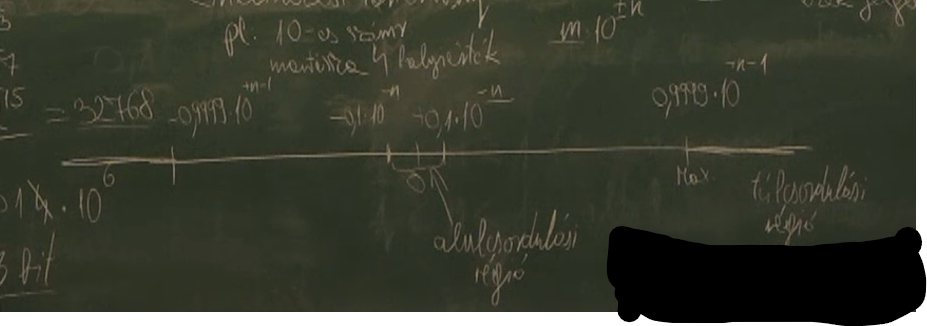
\includegraphics[width=0.8\textwidth]{csord}
    \centering
    \caption{Alul- és túlcsordulási régiók}
    \label{fig:csord}
\end{figure}

Az architektúrának biztosítania kell a túlcsordulás felismerését, jelzését és kezelését.

Az architektúra lehetőségei túlcsordulás esetén:
\begin{itemize}
    \item kijelzi a túlcsordulást és beállítja a legnagyobb megengedett értéket
    \item kijelzi a túlcsordulást és előjeles végtelent jelez ki
\end{itemize}
Alulcsordulás esetén:
\begin{itemize}
    \item kijelzi az alulcsordulást és nullára konvertál
    \item kijelzi az alulcsordulást denormalizált számot jelzi ki
\end{itemize}
A kijezést flagek segítségével teszi.

A szabvány előírja, hogy ha a mantissza nulla, a karakterisztikának is nullának kell lennie.

\section{Pontosság növelése}
Probléma, hogy a tízes számrendszerben pontosan megadható számok egy része kettes számrendszerben végtelen tizedes törtként ábrázolható (pl. 0.3).
A pontosság növelésére alkalmazott módszerek:
\begin{itemize}
    \item rejtett bit használata: a mantissza tört utáni részénél az első számjegy (bit) mindig 1, így nincs információtartalma. Ezért azt nem tároljuk, így egy bittel pontosabb számot tudunk tárolni.
    \item őrző bitek: a szabvány elvárása, hogy a pontatlanság kisebb legyen, mint a normalizált eredmény legkisebb számjegye. Probléma, hogy normalizáláskor értékes biteket veszíthetünk el, ezért a CPU-n belül a regiszterek több biten tárolják a mantisszát. Általában +3-15 bit. Ezek az őrző bitek, amik a memóriában tárolás során nem jelennek meg. Az őrző bitek felhasználása:
    \begin{itemize}
        \item a rejtett bit balra léptetésekor értékes bitet tudunk beléptetni
        \item tárolási formátum kérésekor kerekített értéket tárolhatunk
        \item normalizáláskor értékes biteket tudunk felhasználni
    \end{itemize}
\end{itemize}

\section{Lebegőpontos műveletvégzés jellemzői}
\begin{itemize}
    \item kódolás: mantissza kódolása 2-es komplemens, karakterisztika kódolása többletes kódolással. Ennek oka, hogy a többletes kód kialakítása gyorsabb, de elsősorban csak összeadás és kivonás elvégzésére alkalmas. Szorzást, osztást egyszerűbb kettes komplemenssel kódolt számokon könnyebb.
\end{itemize}

\section{IEEE 754 további jellemzői}
A szabvány fő célja a kompatibilitás megteremtése különböző CPU-k között.
A hardvernek és a szoftvernek együtt kell biztosítania a szabványnak való megfelelést.

A szabvány legfontosabb fejezetei:
\begin{itemize}
    \item adattípus
    \item formátumok
    \begin{itemize}
        \item szabványos (háttértáron tárolás)
        \begin{itemize}
            \item egyszeres pontosságú (32 bit)
            \item kétszeres pontosságú (64 bit)
        \end{itemize}
        \item kiterjesztett (CPU-n belül)
        \begin{itemize}
            \item egyszeres pontosságú (32 bit)
            \item kétszeres pontosságú (64 bit)
        \end{itemize}
    \end{itemize}
    \item műveletek
    \item kerekítések
    \item kivételek kezelése
\end{itemize}

A szabvány által meghatározott műveletek:
\begin{itemize}
    \item négy aritmetikai művelet
    \item maradékképzés
    \item gyökvonás
    \item bináris-decimális konverzió
    \item értelmezett a végtelennel való műveletvégzés
    \item kerekítések
    \begin{itemize}
        \item legközelebbire kerekítés
        \item nullára kerekítés (őrző bitek levágása)
        \item kerekítés pozitív végtelen felé
        \item kerekítés negatív végtelen felé
    \end{itemize}
\end{itemize}

A kivételek felbukkanása általában megszakítást eredményez.
Kivételek lehetnek pl. overflow, underflow, nullával osztás, gyökvonás negatív számból.

Először a lebegőpontos egységek koprocesszorokban voltak, később az Intel 80486 CPU-nál már a processzorba volt integrálva.

\section{Műveletek megvalósítása}

\begin{itemize}
    \item A+B: azonos hatványra hozás és összeadás
    \item A*B: A és B mantisszájának szorzása és a karakterisztikák összeadása
\end{itemize}
A szorzásnál fontos, hogy a két művelet párhuzamosan elvégezhető, így növelhető a sebesség.
Ennek a megvalósítása dedikált FP műveletvégzővel történik: egy adatbuszon keresztül a mantissza a mantissza egységbe, a karakterisztika pedig a karakterisztika egységbe kerül, a végeredményt pedig a vezérlő rakja össze.

\section{BCD számábrázolás}
Megjelenésének fő oka a fixpontos és a lebegőpontos számok pontatlansága.
Elsősorban adminisztratív és tudományos alkalmazásoknál használják (pl. számológépek).
A lebegőpontos konvertálás lehet pontatlan, de a kódolás pontos megfeleltetés, nincs kerekítés.

BCD kódolásnál minden számjegyet 4 biten ábrázolunk.
Mivel 4 bit 16 féle értéket vehet fel, keletkezik 6 darab érvénytelen tetrád, ami nincs használatban BCD kódolásnál.

\subsection{Ábrázolási formátumok}
\begin{itemize}
    \item zónázott: 1 byte = 1 számjegy, minden tetrádot megelőz 4 zóna bit
    \item pakolt: 1 byte = 2 számjegy (pl. Intel)
\end{itemize}

\subsection{Műveletvégzés logikai szinten}
Példa: 8+7=15.
BCD kódolva ez 1000+0111=1111, ami egy érvénytelen tetrádot eredményez, így 10-et ki kell vonni belőle (azaz hozzáadunk -10-et).
Kettes komplemens esetben 1010 invertálva 0101, majd hozzáadva egyet 0110.
Ezzel előáll az 5 mint eredmény.

\subsection{Műveletvégzés áramköri szinten}
A megvalósításhoz szükség van 4 db teljes összeadóra.
Az áramkörnek el kell végeznie az érvénytelen tetrádok kezelését is.
Az előző példánál az áramkör működése:
\begin{figure}[H]
    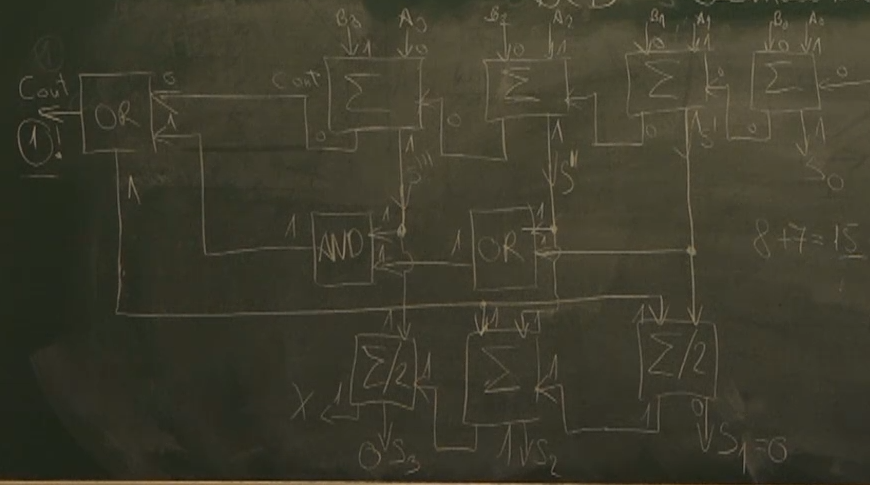
\includegraphics[width=0.8\textwidth]{bcd}
    \centering
    \caption{BCD összeadó áramkör}
    \label{fig:bcd}
\end{figure}

\subsection{Összegzés}
A BCD kódolás előnye tehát, hogy teljesen pontos, viszont jelentősen több helyet foglal, mint a lebegőpontos számok, valamint lassabb a végrehajtás is sok esetben.
A BASIC programnyelv ezt használja.

\section{Az ALU egyéb műveletei}
Az aritmetikai műveleteken kívül egyéb műveleteket is ellát az ALU, ezek általában egyszerűbb áramköröl segítségével megoldhatók.
\begin{itemize}
    \item Boole műveletek (mind a 16 fajta) pl.:
    \begin{itemize}
        \item AND
        \item NOR
        \item XOR
    \end{itemize}
    \item léptetés
    \item invertálás
    \item komparálás (feltételes ugrás)
    \item LOAD/STORE címszámítás - valós időben címet generál a MAR számára
    \item karakteres műveletek
\end{itemize}

\end{document}
